\documentclass[12pt,a4paper]{article}
\usepackage[utf8]{inputenc}
\usepackage[a4paper, total={6in, 8in},headsep=60pt,textheight=650pt]{geometry}
\usepackage{amsmath}
\usepackage{amssymb}
\usepackage{fancyhdr}
\usepackage{pgfplots}
\usepackage{graphicx}
\usepackage{tikz}
\usepackage{mhchem}
\usepackage[many]{tcolorbox}

\graphicspath{ {../images/} }

\pgfplotsset{compat=1.16}
\title{Math test}
\author{Dipam Sen}
\pagestyle{fancy}
\renewcommand{\headrulewidth}{0pt}
\renewcommand{\footrulewidth}{0pt}

\usetikzlibrary{shapes.geometric}
\usetikzlibrary{shapes.misc}

\newtcolorbox{note}{
  colback=black!5!white,colframe=black!75, adjusted title=\textbf{Note}
}
\newtcolorbox{question}{
  colback=red!5!white,colframe=red!75,  fontupper=\bfseries
}
\usetikzlibrary{decorations.markings}


\fancyhf{}
\chead{
  
\includegraphics[scale=0.1]{funplanet}\\
}
\cfoot{
  Fun Planet
}
\rfoot{
  Page \thepage
}
\newcommand{\headers}[2]{\lhead{#1\\[2\baselineskip]}\rhead{#2\\[2\baselineskip]}}
\newcommand{\answer}{\tcblower}


\begin{document}

\headers{Chemistry}{Atomic Structure}
\begin{center}
  \huge \textbf{Atomic Structure}
\end{center}

\textbf{Atom:} The smallest particle of matter which may or may not stably exist, but can take part in chemical reactions.


\section*{Dalton's Atomic Theory}
\begin{itemize}
  \item Matter is made up of a smallest indivisible particle called atom.
  \item Atoms of same elements are alike in all aspects and atoms of different elements are different in all aspects.
  \item Atoms can neither be created nor be destroyed. In a chemical reaction, atoms are exchanged to form molecules.
\end{itemize}


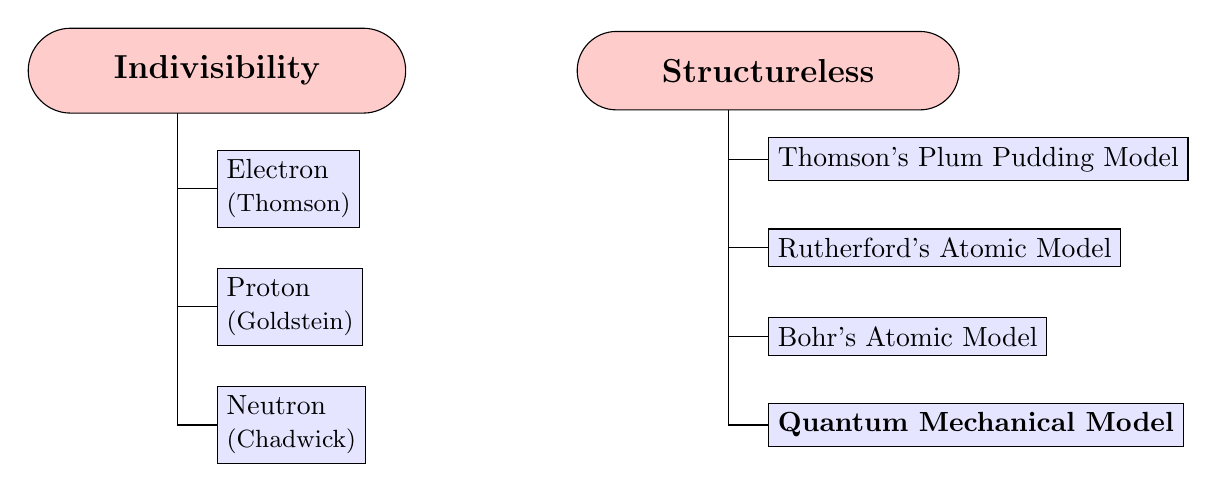
\begin{tikzpicture}
  \draw (-0.5, 0) |- (0, -1.5);
  \draw (-0.5, 0) |- (0, -3);
  \draw (-0.5, 0) |- (0, -4.5);
  \node at (0,0)  [rounded rectangle,draw, fill=red!20,inner ysep=1em, inner xsep=3em] {{\large\bfseries Indivisibility}};
  \node at (0,-1.5)  [draw,anchor=west, fill=blue!10,align=left] {Electron\\\small{(Thomson)}};
  \node at (0,-3)  [draw,anchor=west, fill=blue!10,align=left] {Proton\\\small{(Goldstein)}};
  \node at (0,-4.5)  [draw,anchor=west, fill=blue!10,align=left] {Neutron\\\small{(Chadwick)}};

  \draw (6.5, 0) |- (7, -1.125);
  \draw (6.5, 0) |- (7, -2.25);
  \draw (6.5, 0) |- (7, -3.375);
  \draw (6.5, 0) |- (7, -4.5);
  \node at (7,0)  [rounded rectangle,draw, fill=red!20,inner ysep=1em, inner xsep=3em] {{\large \bfseries Structureless}};
  \node at (7,-1.125)  [draw,anchor=west, fill=blue!10,align=center] {Thomson's Plum Pudding Model};
  \node at (7,-2.25)  [draw,anchor=west, fill=blue!10,align=center] {Rutherford's Atomic Model};
  \node at (7,-3.375)  [draw,anchor=west, fill=blue!10,align=center] {Bohr's Atomic Model};
  \node at (7,-4.5)  [draw,anchor=west, fill=blue!10, align=center] {\bfseries Quantum Mechanical Model};
\end{tikzpicture}

\section*{Discovery of an Electron}

\subsection*{Discharge Tube Experiment / Cathode Ray Tube}

\begin{figure}
  \centering
  \begin{tikzpicture}
    \node (crt) at (0, 0) {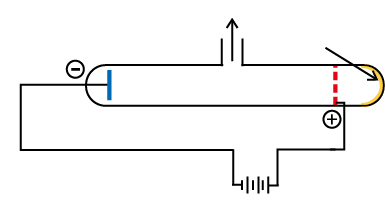
\includegraphics[width=0.65\textwidth]{cathoderaytube}};
    % \draw[step=1cm,gray,very thin] (-7.5, -3) grid (7.5,3);
    \draw (1, 2.7) node {To Vacuum};
    \draw (2.5, 1.8) node [anchor=west] {fluoroscent material (ZnS)};
    \draw (5.2, 1.5) node [color=green!60!black, anchor=north west, align=center] {\small greenish\\\small yellow\\\small glow};
    \draw (3.4, -0.25) node [anchor=east] {\small Perforated anode};
    \draw (-3.2, 1) node [anchor=east] {\small Cathode};
    \draw (1.5, -2.2) node [anchor=north] {10 kV};
    \draw (-7, 2.5) node [anchor=north west] {Pressure = $10^{-4}$ to $10^{-5}$ mm Hg};

    \foreach\y in {0.25, 0.45, ..., 0.9}
    \draw[decoration={markings,mark=at position 1 with {\arrow[scale=2]{>}}},
      postaction={decorate},
      shorten >=0.4pt, ultra thin, blue, dashed] (-2.1, \y) -- (3.6, \y);

    \draw (1, 0.5) node {Cathode rays};

    \draw (-7, -1.2) node [align=left, anchor=north west] {
      $
        \left.
        \begin{tabular}{c}
          Low Pressure \\ High Voltage
        \end{tabular}
        \right\} \text{Gases ionise}
      $
    };
  \end{tikzpicture}
  \caption{JJ Thomson's Cathode Ray Tube Experiment} \label{fig:M1}
\end{figure}

\subsubsection*{Characteristics of Cathode Rays}
\begin{enumerate}
  \item They are originated from the cathode and move towards the anode. Therefore they are called cathode rays.
  \item Cathode rays are made up of negatively charged materiallistic particles, which were later called electrons.
  \item Cathode rays travel in a straight line and is deflected by electric and magnetic fields.
  \item Cathode rays produce heating effect and they can produce x-rays on striking on surface of hard metal.
\end{enumerate}

\begin{note}
  \begin{itemize}
    \item Gases are ionised at low pressure and high voltage.
    \item Cathode rays consist of electrons ejected from cathode and evolved from ionisation of gases.
  \end{itemize}
\end{note}

\subsubsection*{Specific Charge ($\frac em$ ratio) for Electron}

$$\left(\frac em\right)_{e^-}=1.7588\times 10^{11} \mathrm{C\ kg^{-1}}$$

Specific Charge does not depend on the nature of gas or nature of electrodes.

\subsubsection*{Charge and Mass of Electron}

The charge of an electron was discovered by Millikan's Oil Drop Experiment.
\begin{align*}
  \text{Charge on an Electron} & = -1.6\times 10^{-19} \mathrm{C} \\
  \text{Mass of an Electron}   & = 9.1\times 10^{-31} \mathrm{kg}
\end{align*}

\section*{Discovery of Proton}

% image

\subsection*{Characteristics of Anode Rays}

\begin{enumerate}
  \item Anode rays move from the anode to cathode.
  \item They travel in a straight line.
  \item The $e/m$ values of an anode ray depend on the
        \begin{itemize}
          \item nature of gas
          \item nature of electrodes
        \end{itemize}
  \item Anode rays consist of positively charged materialistic particles, which in case of Hydrogen is called a proton.
\end{enumerate}

$$\left(\frac em\right)_{p^+}=9.6\times 10^{7} \mathrm{C\ kg^{-1}}$$

\begin{align*}
  \text{Charge on a Proton} & = +1.6\times 10^{-19} \mathrm{C}  \\
  \text{Mass of a Proton}   & = 1.67\times 10^{-27} \mathrm{kg}
\end{align*}


\subsection*{Discovery of Neutron}
(Chadwick)

$$\ce{_4^9Be + _2^4He -> _6^12C + _0n^1}$$

When a lighter nuclei is bombarded with energetic $\alpha$ particles, a stable nuclei and an unidentified particle is observed. This particle was later known as neutron.


\begin{align*}
  \text{Charge on a Neutron} & = 0                               \\
  \text{Mass of a Neutron}   & = 1.67\times 10^{-27} \mathrm{kg}
\end{align*}


\subsubsection*{Specific Charge Values}

\begin{align*}
   & e^- =1.76\times 10^{11} \mathrm{\ C\ kg^{-1}}   \\
   & p = 9.6\times 10^{7} \mathrm{\ C\ kg^{-1}}      \\
   & \alpha = 4.8\times 10^{7} \mathrm{\ C\ kg^{-1}} \\
   & n = 0 \mathrm{\ C\ kg^{-1}}
\end{align*}

$$\boxed{n<\alpha<p<e^-}$$

\begin{question}

  Q) Find the ratio of $e/m$ of an electron and $\alpha$ particle.

  \answer

  \begin{align*}
     & = \frac{1.76\times 10^{11} \mathrm{\ C/kg}}{4.8\times 10^{7} \mathrm{\ C/kg}} \\
     & = 3.67 \times 10^3
  \end{align*}

\end{question}

\begin{question}

  Q) An oil drop has $-6.39\times 10^{-19}$ C of charge. Find the number of electrons.

  \answer

  \begin{align*}
    n & = \frac{6.39\times 10^{-19} \mathrm{\ C}}{1.6\times 10^{-19} \mathrm{\ C}} \\
      & = 4 \text{ electrons}
  \end{align*}

\end{question}

\section*{Thomson's Plum Pudding Model}

% image

According to Thomson, atoms are assumed to be a sphere in which positive charge is uniformly distibuted and electrons are embedded in this positively charged sphere.

\section*{Rutherford's Gold Foil Experiment}

% image

\begin{enumerate}
  \item Most $\alpha$ particles passed through the gold foil without any deflection.
  \item A few $\alpha$ particles deflected to a very small angle.
  \item Rarely, a very few $\alpha$ particles deflected to a very large angle, i.e. bounced back.
\end{enumerate}

\subsubsection*{Rutherford's Conclusions}

\begin{enumerate}
  \item An atom has a lot of empty space
  \item An atom has a positively charged core at its centre, which was later called the nucleus.
  \item The whole mass of the atom is concentrated at the positively charged centre.
\end{enumerate}

\subsubsection*{Drawback of Thomson's Atomic Model}
Thomson's model was unable to explain the Rutherford's Gold Foil Experiment.

\subsubsection*{Rutherford's Atomic Model}
According to Rutherford,

\begin{enumerate}
  \item All the positive charge and mass of an atom is concentrated in a very small region called the nucleus.
  \item The size of the nucleus (diameter) is about $10^{-15} \mathrm{\ m}$, which is very small as compared to the diameter of the atom, $10^{-10} \mathrm{\ m}$.

        $$\boxed{R_N=R_0 A^{1/3}} = 1.25\times 10^{-15} A^{1/3}$$

  \item  The electrons equal in number to the net nuclear charge revolve around the nucleus.
  \item The centrifugal force arising due to the circular motion of the electrons is balanced by the electrostatic force of attraction.

        % image | eqn

        $$F_{\text{electrostatic}}=\frac{Kq_1q_2}{r^2}$$
        $$F_{\text{centrifugal}}=\frac{mv^2}{r}$$

\end{enumerate}

\end{document}
